\documentclass[10pt]{exam}
\usepackage[phy]{template-for-exam}
\usepackage{tikz}
\usetikzlibrary{shadings,shadows}

\title{Circular \#4}
\author{Rohrbach}
\date{\today}

\begin{document}
\maketitle

\newcommand{\printdata}{
  \begin{center}
    \begin{tabular}{ll}
      \hline
      Reference Data  & \\
      \hline
      Mass of Earth   & \SI{5.98e24}{\kilo\gram} \\
      Radius of Earth & \SI{6.38e6}{\meter}      \\
      Mass of Moon   & \SI{7.35e22}{\kilo\gram} \\
      Radius of Moon & \SI{1.74e6}{\meter}      \\
      \hline
    \end{tabular}
  \end{center}
}

\printdata

\begin{questions}

\question
	A satellite orbits the earth at a distance 1,120 km (\SI{1.12e6}{\meter}) {\bf above the Earth's surface}.  If the force of gravity acting on the satellite is \SI{2100}{\newton}, what is the mass of the satellite? (\emph{Hint:} think carefully about what the radius is.)
  
  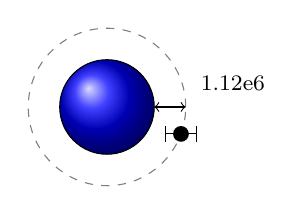
\begin{tikzpicture}
    \draw[shading=ball] (0,0) circle (.6);
    \draw[dashed,gray] (0,0) circle (1);
    \node[fill=white] at (1.6,.3)
      {\footnotesize \SI{1.12e6}{\meter}};
    \draw[<->] (.6,0) -- (1,0);


    \begin{scope}
      \fill (340:1) coordinate (satellite) 
        circle (0.1);
      \draw (satellite) 
        -- ++(.2,0) ++(0,.1) -- ++ (0,-.2);
      \draw (satellite) 
        -- ++(-.2,0) ++(0,.1) -- ++ (0,-.2);
    \end{scope}

  \end{tikzpicture}
  
  \vs[3]

\question
	A astronaut has a mass of 92 kg. 

  \begin{parts}
    \part
      What is the force of gravity between the astronaut and the earth? (Use $F_G=Gm_1 m_2/d^2$.)

      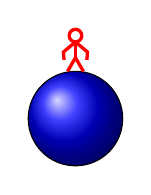
\begin{tikzpicture}
        \draw[shading=ball] (0,0) circle (.6);

        \begin{scope}[
            red,
            very thick
          ]
          \def\headsize{0.08}
          \draw (0,.6) 
          ++(-.1,0) coordinate (left foot) --
          ++(60:.2) coordinate (waist) --
          ++(-60:.2) coordinate (right foot);
  
          \draw (waist)
            -- ++(90:.2) coordinate (neck);
          \draw (neck) 
            ++(90:\headsize) circle (\headsize);
          \draw (neck)
            -- ++(-40:0.2) coordinate (right elbow)
            -- ++(-95:0.1) coordinate (right hand);
          \draw (neck)
            -- ++(-140:0.2) coordinate (left elbow)
            -- ++(-85:0.1) coordinate (left hand);
        \end{scope}
      \end{tikzpicture}

      \vs

    \part
     Let's try it a different way.  What is the astronaut's weight on earth using the equation $F_G=mg$?
     \vs[2]

     \part
     The astronaut now travels to the moon.  What is the force of gravity between the astronaut and the moon when he stands on its surface? (Use $F_G=Gm_1 m_2/d^2$.)

     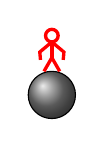
\begin{tikzpicture}
       \draw[shading=ball,ball color=gray] (0,0.3) circle (.3);

       \begin{scope}[
           red,
           very thick
         ]
         \def\headsize{0.08}
         \draw (0,.6) 
         ++(-.1,0) coordinate (left foot) --
         ++(60:.2) coordinate (waist) --
         ++(-60:.2) coordinate (right foot);
 
         \draw (waist)
           -- ++(90:.2) coordinate (neck);
         \draw (neck) 
           ++(90:\headsize) circle (\headsize);
         \draw (neck)
           -- ++(-40:0.2) coordinate (right elbow)
           -- ++(-95:0.1) coordinate (right hand);
         \draw (neck)
           -- ++(-140:0.2) coordinate (left elbow)
           -- ++(-85:0.1) coordinate (left hand);
       \end{scope}
     \end{tikzpicture}

     \vs

   \part
    Use the equation $F_G=mg$ to figure out what $g$ (the acceleration of gravity) is on the surface of the
    \vs[2]

  \end{parts}
	





\end{questions}

\end{document}